% !TeX program = xelatex
% !BIB program = bibtex
% 博士必须给章、节、三级标题提供英文译名：\chapter{中文}[English]
\documentclass[type=doctor,degreeType=professional]{suepthesis}
\SUEPSetup{
  cover = {date = 2026年6月},
  info = {
    title = 面向新能源的电力系统优化研究,
    titleEn = {Optimization of Power Systems with Renewable Energy},
    author = 张三,
    studentId = 20260001,
    supervisor = 李四教授,
    institution = 电气工程学院,
    institute = 电气工程学院,
    major = 能源动力,
    degree = 工程博士,
    classification = TM73,
    classifiedLevel = 公开,
    finalizationDate = 2026年6月1日,
    keywords = {电力系统,新能源,优化调度,储能},
    keywordsEn = {Power systems,Renewable energy,Optimal scheduling,Energy storage},
  }
}
\usepackage{gbt7714}
\SUEPBibliographyStyle
\begin{document}
\MakeCover
\MakeOriginality
\frontmatter
\begin{abstract}
新能源发电的波动性给电力系统运行带来新的挑战。本文以含新能源和储能的电力系统为研究对象，建立考虑功率平衡、设备容量与运行成本的优化模型，分析新能源出力变化对系统调度的影响。

研究采用数学建模与数值分析相结合的方法，通过统一描述发电、负荷和储能设备的运行约束，构建具有可解释性的优化框架。模型以系统运行成本最小为目标，并对储能充放电行为进行约束，以保证调度方案满足设备运行条件。

本文给出模型的主要变量、目标函数和约束关系，并讨论求解结果的物理意义。研究表明，通过协调新能源发电与储能资源，可以改善电力系统的运行方式。所建立的框架为后续开展不确定性分析和多时间尺度协调提供基础。

\end{abstract}
\begin{abstractEn}
Renewable generation introduces new challenges to power system operation. This study develops an optimization model for a power system with renewable generation and energy storage, subject to power balance, capacity limits, and operating constraints.

The model combines mathematical modeling with numerical analysis. Its objective is to minimize system operating costs while coordinating generation, demand, and storage. The physical meaning of the variables and constraints is discussed to support interpretation of the scheduling results.

The main variables, objective function, and constraints are presented, and their physical meaning is discussed. Coordinating renewable generation and energy storage provides a framework for subsequent uncertainty analysis and coordination across multiple time scales.
\end{abstractEn}

\MakeTOC
\mainmatter
\chapter{绪论}[Introduction]
\section{研究背景与意义}[Background and Motivation]
电力系统优化需要综合考虑运行成本与设备约束。本文采用数学模型刻画各设备之间的关系。模型设计参考已有建模与计算方法\supercite{knuth,lamport}。

发电设备、负荷和储能共同构成系统的功率平衡关系。优化过程中需要同时考虑设备容量、运行成本以及储能充放电约束。
\subsection{研究内容}[Research Scope]
研究包括建模、求解和分析三个方面，通过建立变量与约束之间的联系，分析新能源出力变化对系统运行方式的影响。
\section{论文组织结构}[Organization of the Thesis]
第一章介绍研究背景。第二章展示图、表和公式。最后给出结论、参考文献和附录。
\chapter{模型与结果分析}[Model and Results]
\section{优化模型}[Optimization Model]
\subsection{目标函数}[Objective Function]
设决策向量为 $\symbfit{x}$，目标函数和约束为
\begin{equation}\label{eq:model}
  \min_{\symbfit{x}} f(\symbfit{x})
  \qquad \text{subject to } A\symbfit{x}=\symbfit{b}
\end{equation}
式\eqref{eq:model}中，目标函数描述运行成本，等式约束表示系统平衡条件。
\section{非线性构形与物流范围}[Nonlinear States and Logistics]
图\ref{fig:system}描述非线性构形之间的状态转移，图中的刚度曲线反映不同构形在载荷变化下的响应。
\begin{figure}[htbp]
  \centering
  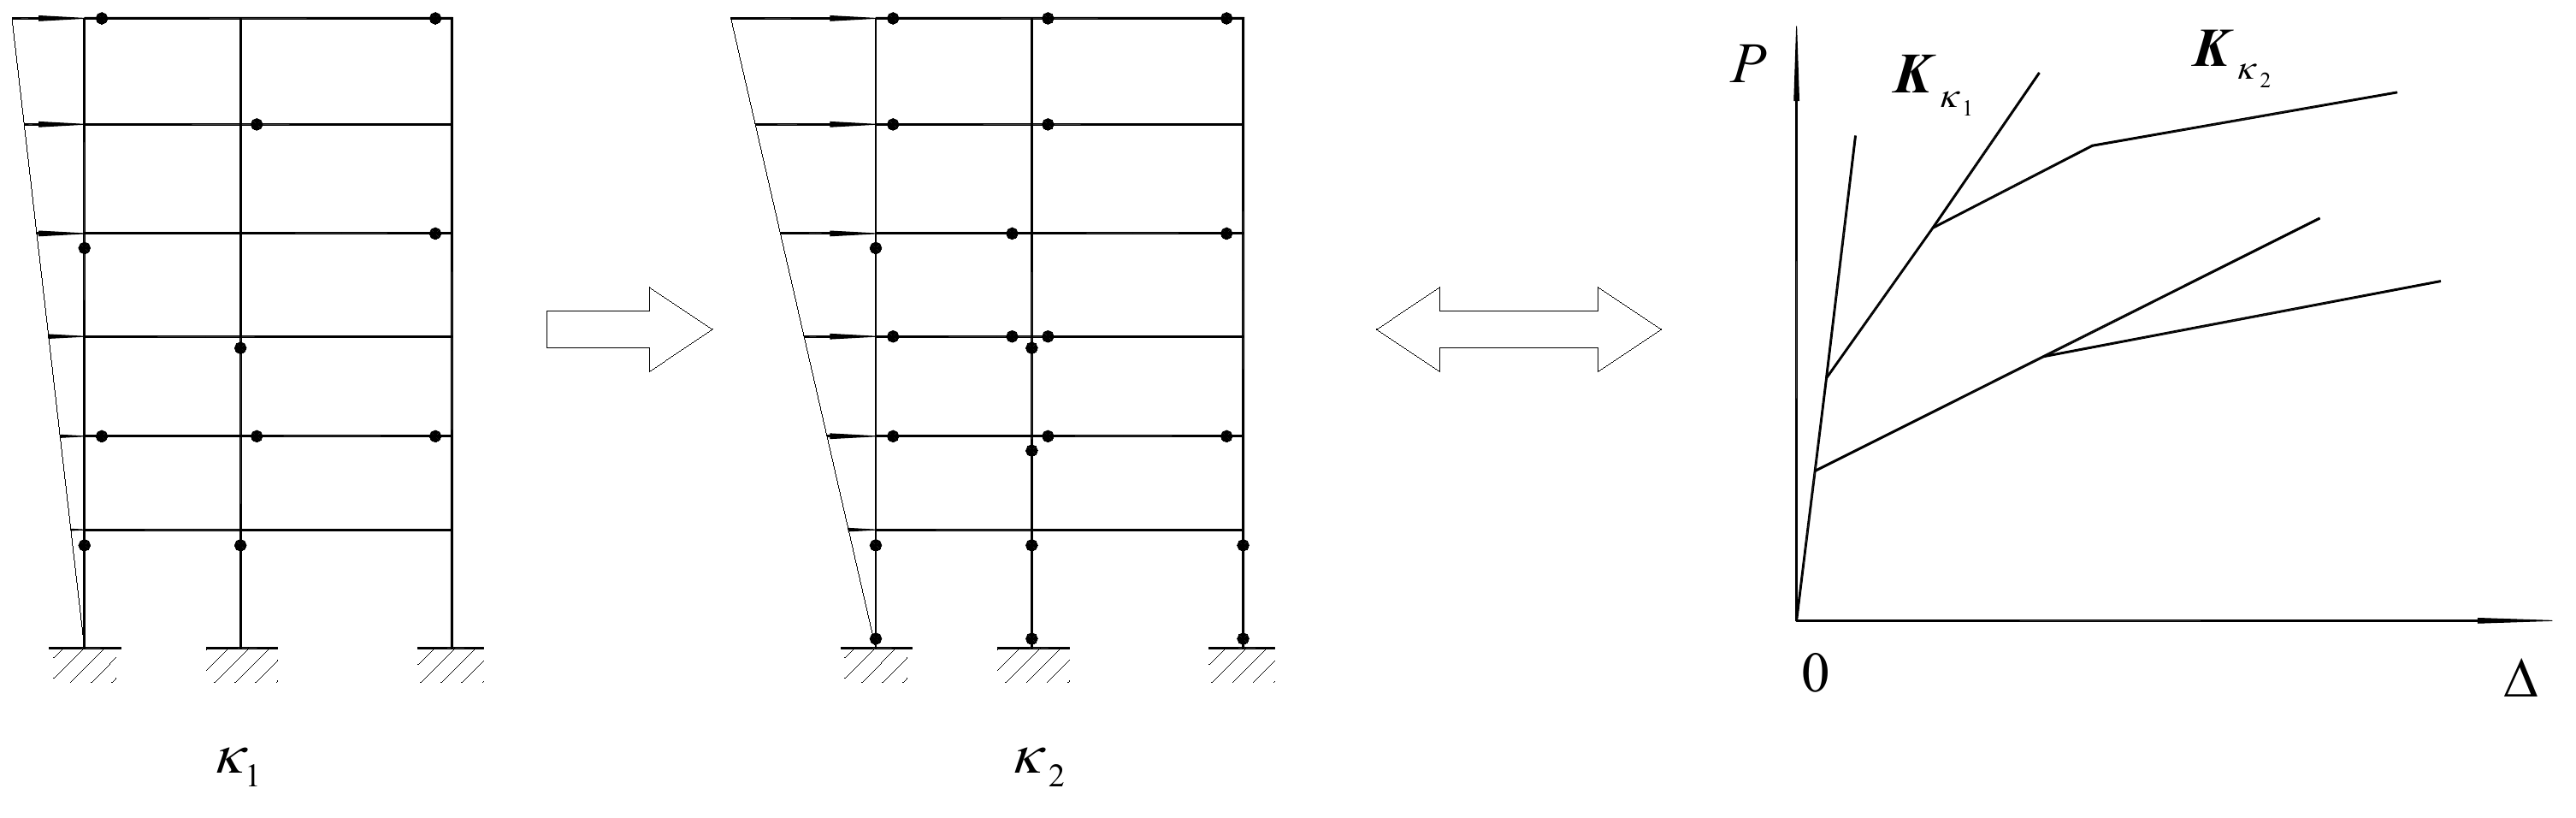
\includegraphics[width=0.85\linewidth]{images/nonlinear-state.png}
  \SUEPCaption{非线性构形状态转移过程示意}{Nonlinear configuration state transition}
  \label{fig:system}
\end{figure}
物流的概念和范围如表\ref{tab:parameters}所示。设备及其原材料在供应商与最终顾客之间流动，规划、实施和控制共同构成这一过程的管理途径。物料流动与存储需要综合考虑效率及成本效益，并适应产品功能、数量、质量和交付时间等需求。
\begin{table}[htbp]
  \centering
  \SUEPCaption{物流的概念和范围}{Conception and scope of Logistics}
  \label{tab:parameters}
  \begin{tabular}{@{}>{\centering\arraybackslash}m{0.20\linewidth}@{}>{\centering\arraybackslash}m{0.70\linewidth}@{}}
    \toprule
    本质 & 过程 \\
    \midrule
    途径或方法 & 规划、实施、控制 \\
    目标 & 效率、成本效益 \\
    活动或作业 & 流动与储存 \\
    处理对象 & 原材料、在制品、产成品、相关信息 \\
    范围 & 从原点（供应商）到终点（最终顾客） \\
    目的或目标 & 适应顾客的需求（产品、功能、数量、质量、时间、价格） \\
    \bottomrule
  \end{tabular}
\end{table}
\subsection{状态响应}[State Response]
系统在时刻 $t$ 的功率平衡满足
\begin{equation}\label{eq:balance}
  P_t^{\mathrm{g}}+P_t^{\mathrm{s}}=P_t^{\mathrm{d}}
\end{equation}

令 $x$ 为状态变量，$a$、$b$、$c$、$d$ 为模型参数。状态响应采用三次项、一次项与反比例项的组合描述：
\begin{equation}
  y = ax^3 + bx + \frac{c}{x} + d
  \label{eq:response}
\end{equation}

\begin{equationnotes}
  \item[$y$] 响应量；
  \item[$a$] 三次项系数；
  \item[$x$] 非零状态变量；
  \item[$b$] 一次项系数；
  \item[$c$] 反比例项系数；
  \item[$d$] 常数项系数。
\end{equationnotes}
式\eqref{eq:response}用于描述不同状态变量取值下的响应变化。

\begin{conclusion}
\section{结论}[Conclusions]
本文完成了新能源电力系统优化模型的建立与分析，刻画了新能源出力、储能状态和功率平衡之间的关系。模型将设备运行约束纳入统一的优化问题，为不同运行条件下的调度分析提供了基础。
\section{进一步工作的方向}[Directions for Future Work]
后续工作可进一步考虑预测误差与多时间尺度协调，并通过不同场景下的运行数据检验模型的适用范围。
\end{conclusion}
\backmatter
\begin{bibprint}
  \bibliography{references}
\end{bibprint}
\begin{appendices}
\chapter{模型参数}[Model Parameters]
模型参数满足以下平衡关系。
\begin{equation} x_1 + x_2 = 1 \end{equation}
\end{appendices}
\begin{acknowledgements}
感谢指导教师和同学对本研究的帮助。
\end{acknowledgements}
\begin{publications}
% 按实际成果填写；示例不虚构个人发表记录。
\end{publications}
\begin{research}
% 按实际科研经历填写；填写方法见手册。
\end{research}
% 书脊单独交给装订人员；需要时取消下一行注释。
% \MakeSpine
\end{document}
